
%
% template for Bachelor thesis
% LIACS
% January 7, 2019
%

\documentclass[12pt]{article}

% include some packages
\usepackage[left=2cm,right=2cm,top=2cm,bottom=3cm]{geometry}
\usepackage{graphicx}
\usepackage{tikz}
\usetikzlibrary{shapes,backgrounds,calc,arrows}
\usepackage{microtype}
\usepackage{amsmath}
% fill in title and author
\usepackage[setpagesize=false,colorlinks=true,linkcolor=blue,urlcolor=red,pdftitle={An Interesting Title for a Thesis},pdfauthor={Your Name}]{hyperref}
\frenchspacing
\setlength{\parindent}{0pt}

\begin{document}

\thispagestyle{empty}


\includegraphics{logoleiden}

\vspace{-2.5cm}\hfill \begin{huge}\textbf{Opleiding Informatica}\end{huge}

\vspace{5cm}
\begin{Large}
\hfill Simplicial Coalgebras

\vspace*{3mm}

\hfill for Concurrent Regular Languages

\vspace*{14mm}

\hfill Hessel Sieburgh
\end{Large}

\vspace*{6.0cm}

\begin{large}

Supervisors:\\
Henning Basold \& 
Marton Hablicsek


\vspace*{2.8cm}
BACHELOR THESIS

\vspace*{5mm}
Leiden Institute of Advanced Computer Science (LIACS)\\
\href{www.liacs.leidenuniv.nl}{\underline{\texttt{www.liacs.leidenuniv.nl}}}\hfill 01/07/2025
\end{large}

\newpage



% abstract and references should fit on one page
\begin{abstract}
\noindent
This is where you write an abstract that concisely summarizes your thesis.
Keep it short. No references here --- exceptions do occur.
\end{abstract}

\bigskip

\thispagestyle{empty}
\tableofcontents
\thispagestyle{empty}
%Some (very few) people like a list of tables:
%\listoftables
%And some (even fewer) like a list of figures:
%\listoffigures

\clearpage
\setcounter{page}{1}

\section{Introduction} \label{introduction}

In this section we give an introduction to the problem addressed in this thesis.


\subsection{The situation}

Sections may include subsections.

To make sure that this document renders correctly, execute these commands:
\begin{quote}
\begin{verbatim}
pdflatex thesis
bibtex thesis
pdflatex thesis
pdflatex thesis
\end{verbatim}
\end{quote}
Here, the \verb|pdflatex| command may need to be executed three times in order to generate the table of contents and so on. 
Note that a good thesis has figures and tables; examples can be found in Figure~\ref{afigure} and Table~\ref{atable}. And every thesis has references, like~\cite{whatagreatpaper}.

\begin{figure}[!htbp]
\begin{center}
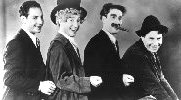
\includegraphics[height=2cm]{marxbrothers2}
\end{center}
\caption{Every thesis should have figures. Source: \href{www.marxbrothers.org}{\underline{\texttt{www.marxbrothers.org}}}.}\label{afigure}
\end{figure}

\begin{table}[!htbp]
\begin{center}
\begin{tabular}{l|l}
Column A & Column B\\
\hline
Point 1 & Good\\
Point 2 & Bad
\end{tabular}
\end{center}
\caption{Every thesis should have tables.}\label{atable}
\end{table}

Final reminder: this template is just an example, if you want you can make adjustments; also discuss with your supervisor which layout he or she likes. But the front page should be as it is now.

TODO: quite a lot!

\subsection{Thesis overview}
It is recommended to end the introduction with an overview of the thesis. This chapter contains the introduction; Section~\ref{definitions} includes the definitions; Section~\ref{relatedwork} discusses related work; Section~\ref{experiments} describes the experiments and their outcome; Section~\ref{conclusions} concludes. By the way, different section titles are certainly possible.

Also, produce a nice sentence with ``bachelor thesis'', LIACS and the names of the supervisors.

\section{Notes}\label{notes}
\paragraph{Connected components}
Let $S$ be a simplicial set with an iPomset label set $L$ and a labeling map $\ell: S \rightarrow L$. Say that $x,y\in S$ are \textit{iPomset neighbors} iff $\ell(x)$ and $\ell(y)$ are equal when disregarding event order.

This gives us path connected components of $S$ where $x\sim y$ (are connected) iff there is a path of neighbors connecting $x$ and $y$.

In this way \[
\begin{pmatrix} a \\ b \end{pmatrix}
\sim 
\{a,b\}
\sim
\begin{pmatrix} b \\ a \end{pmatrix}
\]
 in the figure below.
\begin{figure}[h]
    \centering
    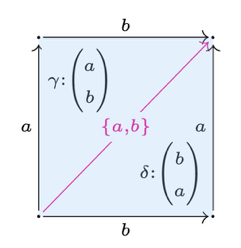
\includegraphics[width=0.3\linewidth]{image.png}
    \caption{equivalence of iPomsets}
    \label{fig:ipomset-equivalence}
\end{figure}
\section{Related Work}\label{relatedwork}

\section{Experiments}\label{experiments}

\section{Conclusions and Further Research}\label{conclusions}

\bibliographystyle{alpha}
\bibliography{bibliography}
\addcontentsline{toc}{section}{References}


%\appendix
%appendices here --- if any

\end{document}
